\mainmatter
\chapter{Introduction}
\label{chap:Introduction}





\section{High-Energy Particle Physics and Standard Model}
Understanding the nature of the particles that constitute matter and radiation is one of the main concerns of science. Particle Physics, also known as High Energy Physics (briefly, `hep'), is the branch of Physics that conducts this ambitious research and its development can be located near the end of $19^\mathrm{th}$ century. Since then, numerous theoretical models have been built in order to predict the outcome of experiments, which can prove their correctness.

At the present, the model that better describes the observed phenomena in hep is the Standard Model, which will be identified with the acronym SM. Since it is the best basis for comparison with experimental results, it will be denoted as `reference model' in the following discussion.

\begin{comment}
\begin{figure}[H]
	\centering
	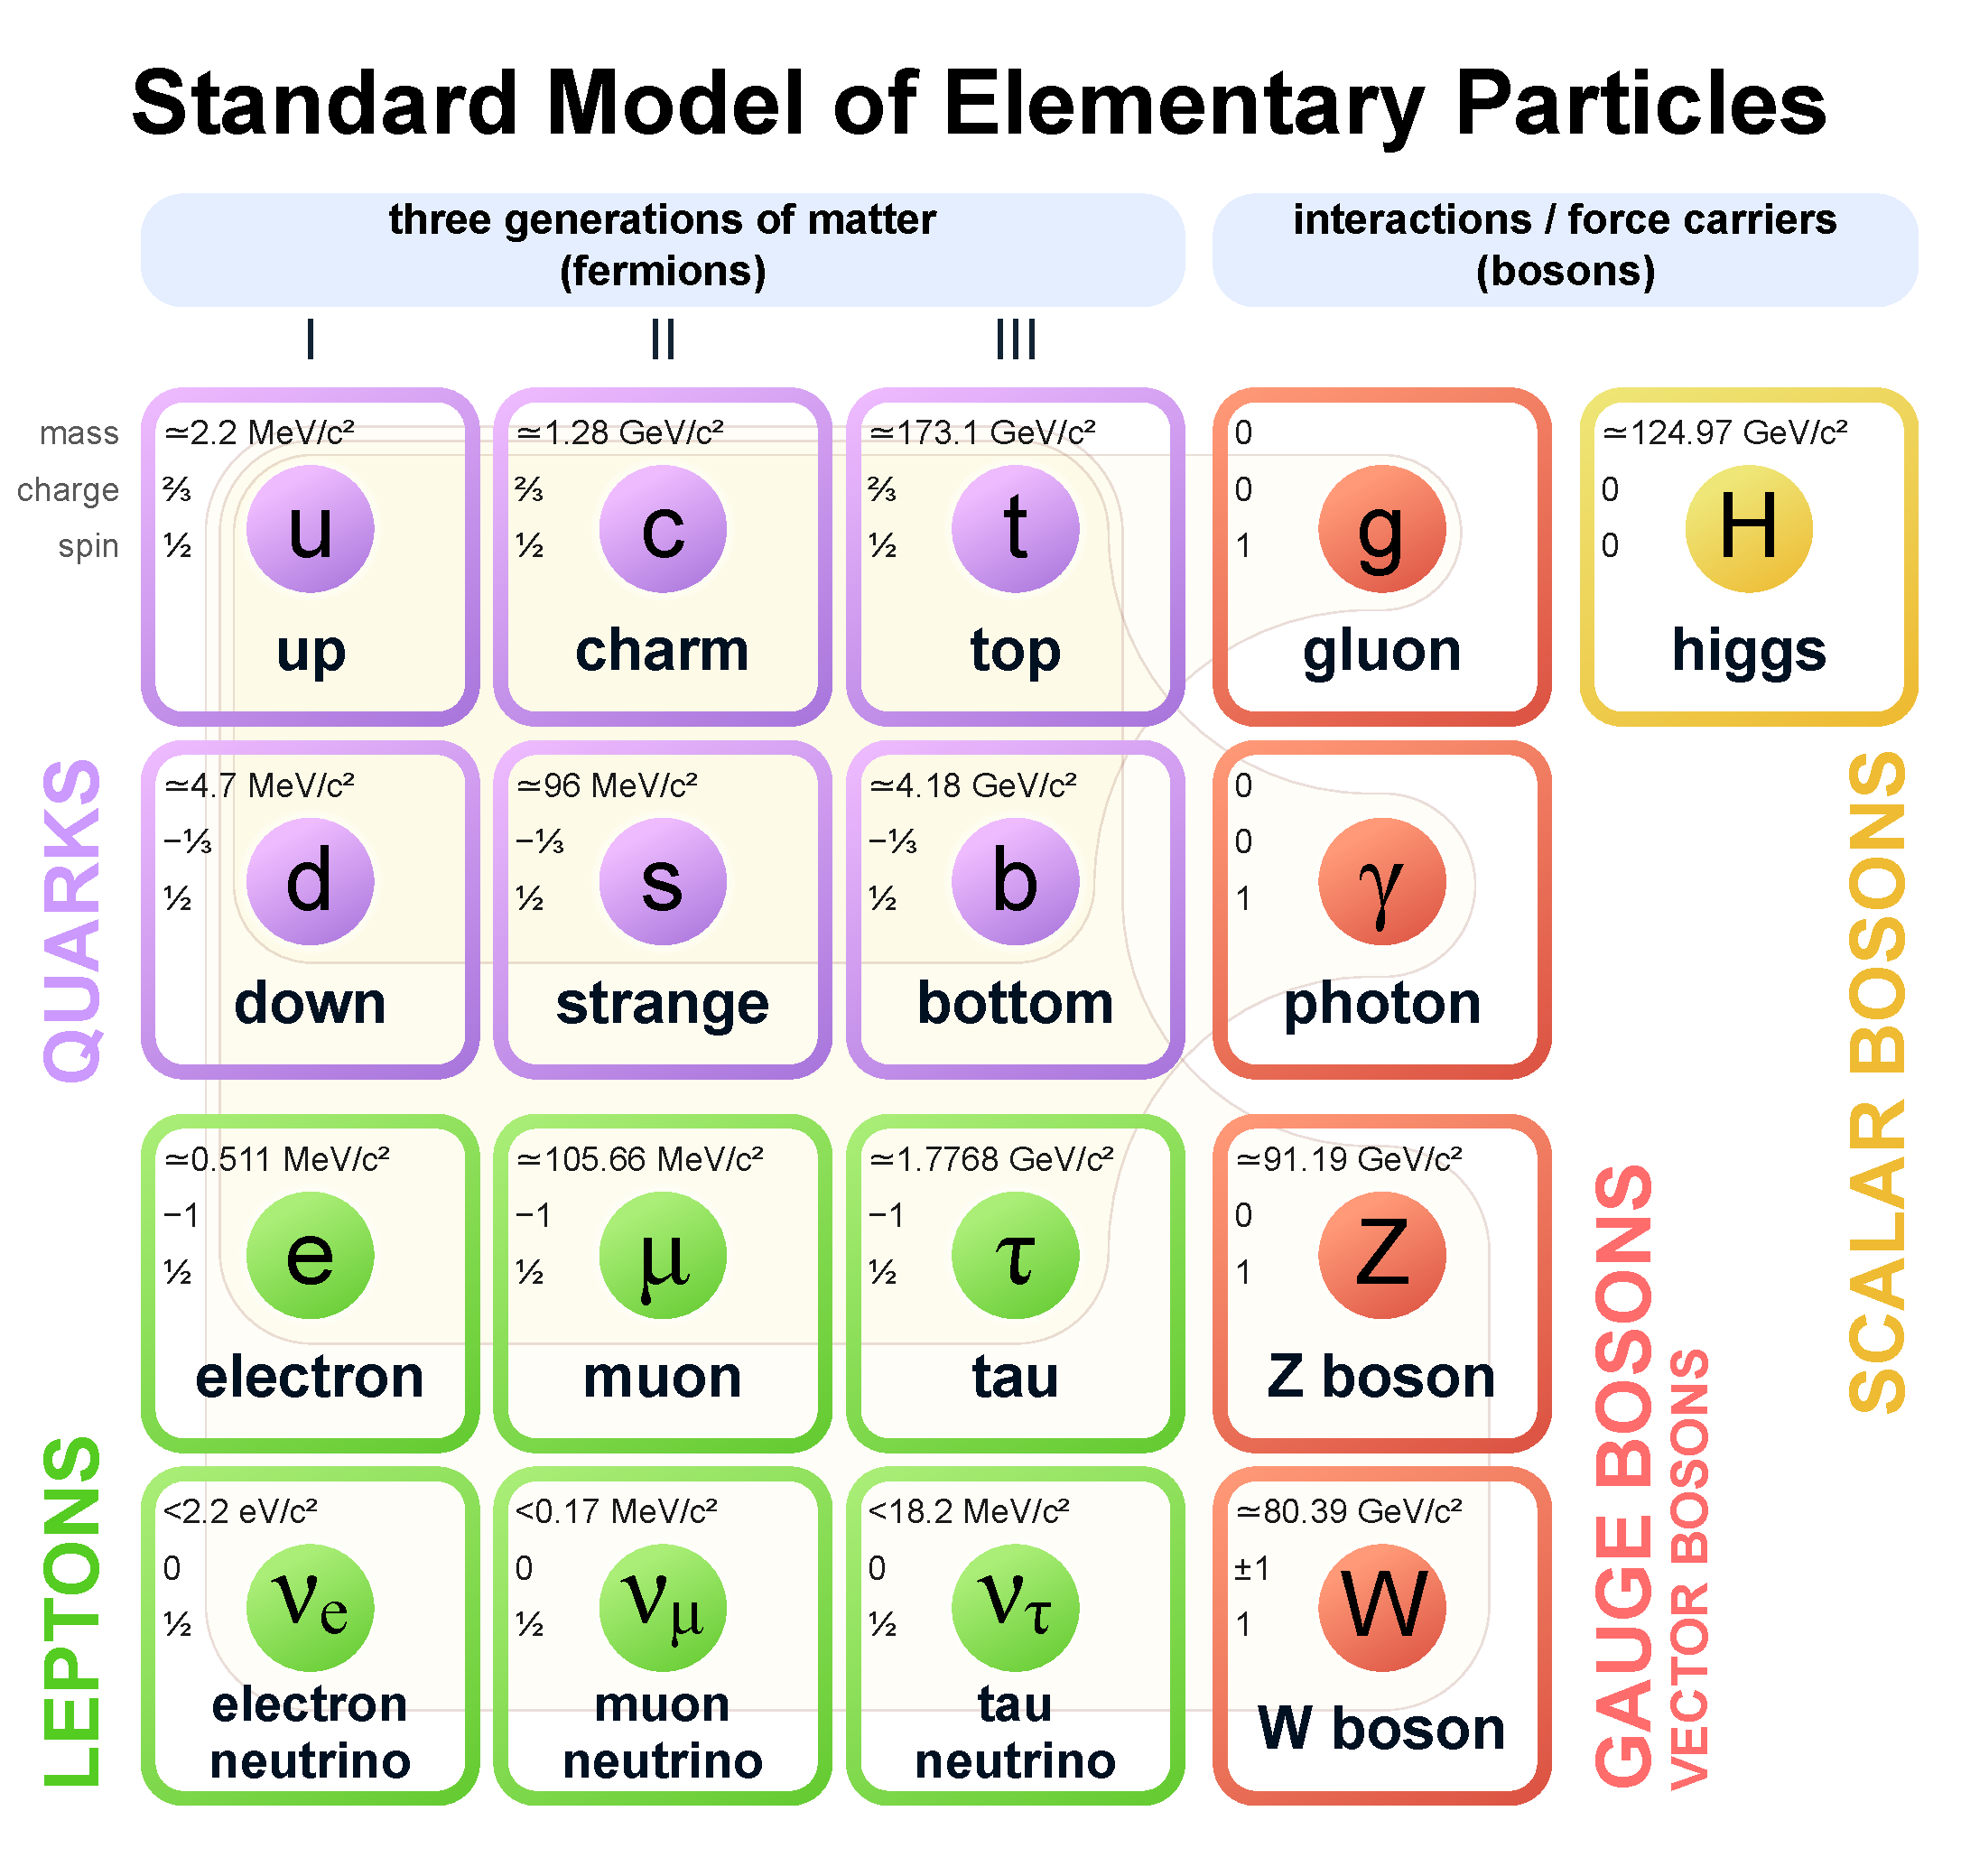
\includegraphics[width=0.4\textwidth]{Images/Introduction/SM_particles.pdf}
	\caption{Standard Model particles.}
	\label{fig:SM_PARTICLES}
\end{figure}
\end{comment}

\begin{figure}[H]
	\centering
	\import{Images/Introduction/}{SM_particles.tex}
	\captionof{figure}{Standard Model of Physics.}
	\label{fig:SM_PARTICLES}
\end{figure}

\noindent
However, althought SM has proved to be extremely successful in predicting a wide variety of particle processes with great accuracy, there are still unexplained phenomena. Among these:
\begin{itemize}
    \item It doesn't explain the canonical theory of gravitation, general relativity, in terms of quantum field theory\footnotemark.
    \footnotetext{It is important to remark that an eventual physical confirmation of a theoretical particle known as a graviton would account for it to a degree.}
    \item Although, as it now stands, it can explain why neutrinos have masses, the specifics of neutrino mass are still unclear.
    \item It doesn't explain the existence of dark matter.
\end{itemize}
Future experiments will be able to explore never observed before phenomena, or they will mesaure known phenomena with a even better accuracy. These facts suggest that new physics (i.e. physical laws not yet established) exists and its research is actually one of the most challenging problems in High Energy Physics.



\subsection{Researches for new physics}
Searching for new physics concretely means searching for discrepancies between observed data and the reference model. This task can be phrased in a more technical way. What we are able to do is taking repeated measurements of a multi-dimensional random variable $x$, experimentally speaking. Then, we can build a Probability Density Function (PDF) using experimental data and test the reference model distribution against the actual data. The first difficulty encountered by seeking this approach is that the true underlying data distribution will be quite similar to the reference one. It means that, if data contain new physics effects, they will be localized in a low-probability region where only a small fraction of event is present, or they will be spread in a large region of the $x$ space.

The most widely employed approach to the problem is to search for specific new physics models. It has the advantage to be physically informative, even if the compatibility of the data with the reference model is confirmed. But there is a critical disadvantage: a statistical test which is designed to be sensitive to one specific hypothesis is typically insensitive to data departures of a different nature from the one expected. So, even if new physics is present in the data, it would not be discovered because it doesn't belong to the class of hypothetical models we are searching for. In Figure \ref{fig:MODEL_DEPENDENT_1} and \ref{fig:MODEL_DEPENDENT_2} there are many examples of excluded models in order to show how difficult it is to search for new physics with this approach.



\subsection{Benefits of a model-independent approach}
After having underlined the difficulties of a model-dependent approach, we can now introduce the strategy of a model-independent approach. But first, it is necessary to clarify the meaning of the expression `model-independent' since it is ill-defined in statistic when it is bound to the concept of hypothesis test. In fact, testing one hypothesis requires an alternative hypothesis to compare with. What we have is basically a set of alternative hypothetical distributions depending on free parameters, also called alternative probability model in statistics. 

In Physics a model is a set of physical laws that make us able to predict these distributions. So we define a certain approach `model-independent' when the alternative distributions don't follow from a physical model, but are selected with other criteria, such as flexibility. It means that the distributions can adapt to the true underlying data distribution for an appropriate choice of the free parameters.

The main reason for which we demand a model-independent approach is the advantage of sensitivity to a large variety of new physics scenarios, including those that are not predicted by any of the models constructed until now.





\section{Machine Learning answer to the problem}
The application of ML techniques to Particle Physics is not the newest addition to the field. The algorithms of this branch are currently applied to aid event selection in the analysis of data given by detectors. In fact, most of the collider events do not produce particles of interest, so making effective measurements requires a filter, in which events producing particles of interest are separated from events producing other particles not involved in the processes we want to study.

\begin{figure}
	\centering
	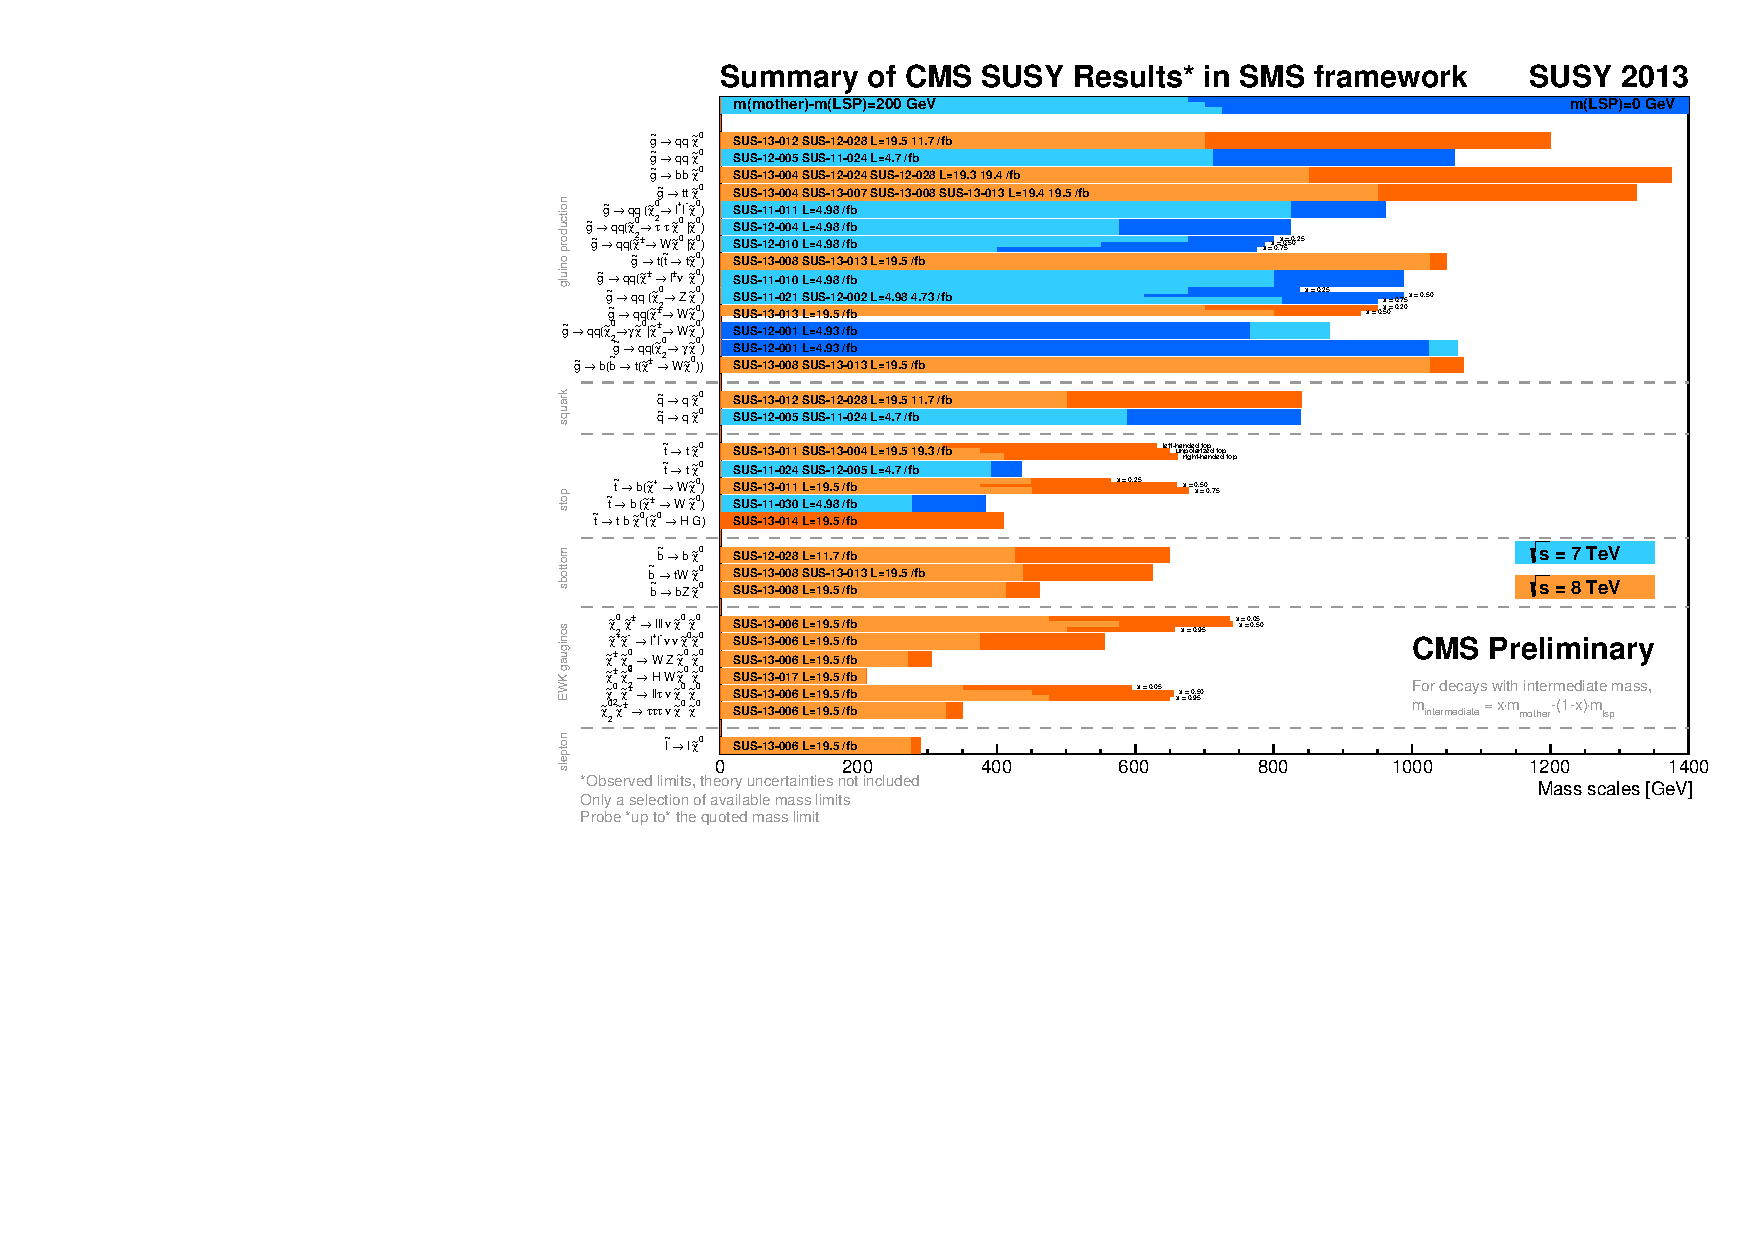
\includegraphics[width=0.9\textwidth]{Images/Introduction/barplot_blue_orange_SUSY2013.pdf}
	\caption{Best exclusion limits for the masses of the mother particles, for RPC scenarios, for m(LSP) = $0~\si{GeV}$ (dark shades) and $m(\text{mother}) - m(\text{LSP}) = 200~\si{GeV}$ (light shades); for each topology, for all results. In this plot, the lowest mass range is $m(\text{mother})=0$, but results are available starting from a certain mass depending on the analyses and topologies. Branching ratios of one are assumed, values shown in plot are to be interpreted as upper bounds on the mass limits \cite{cms_results}.}
	\label{fig:MODEL_DEPENDENT_1}

	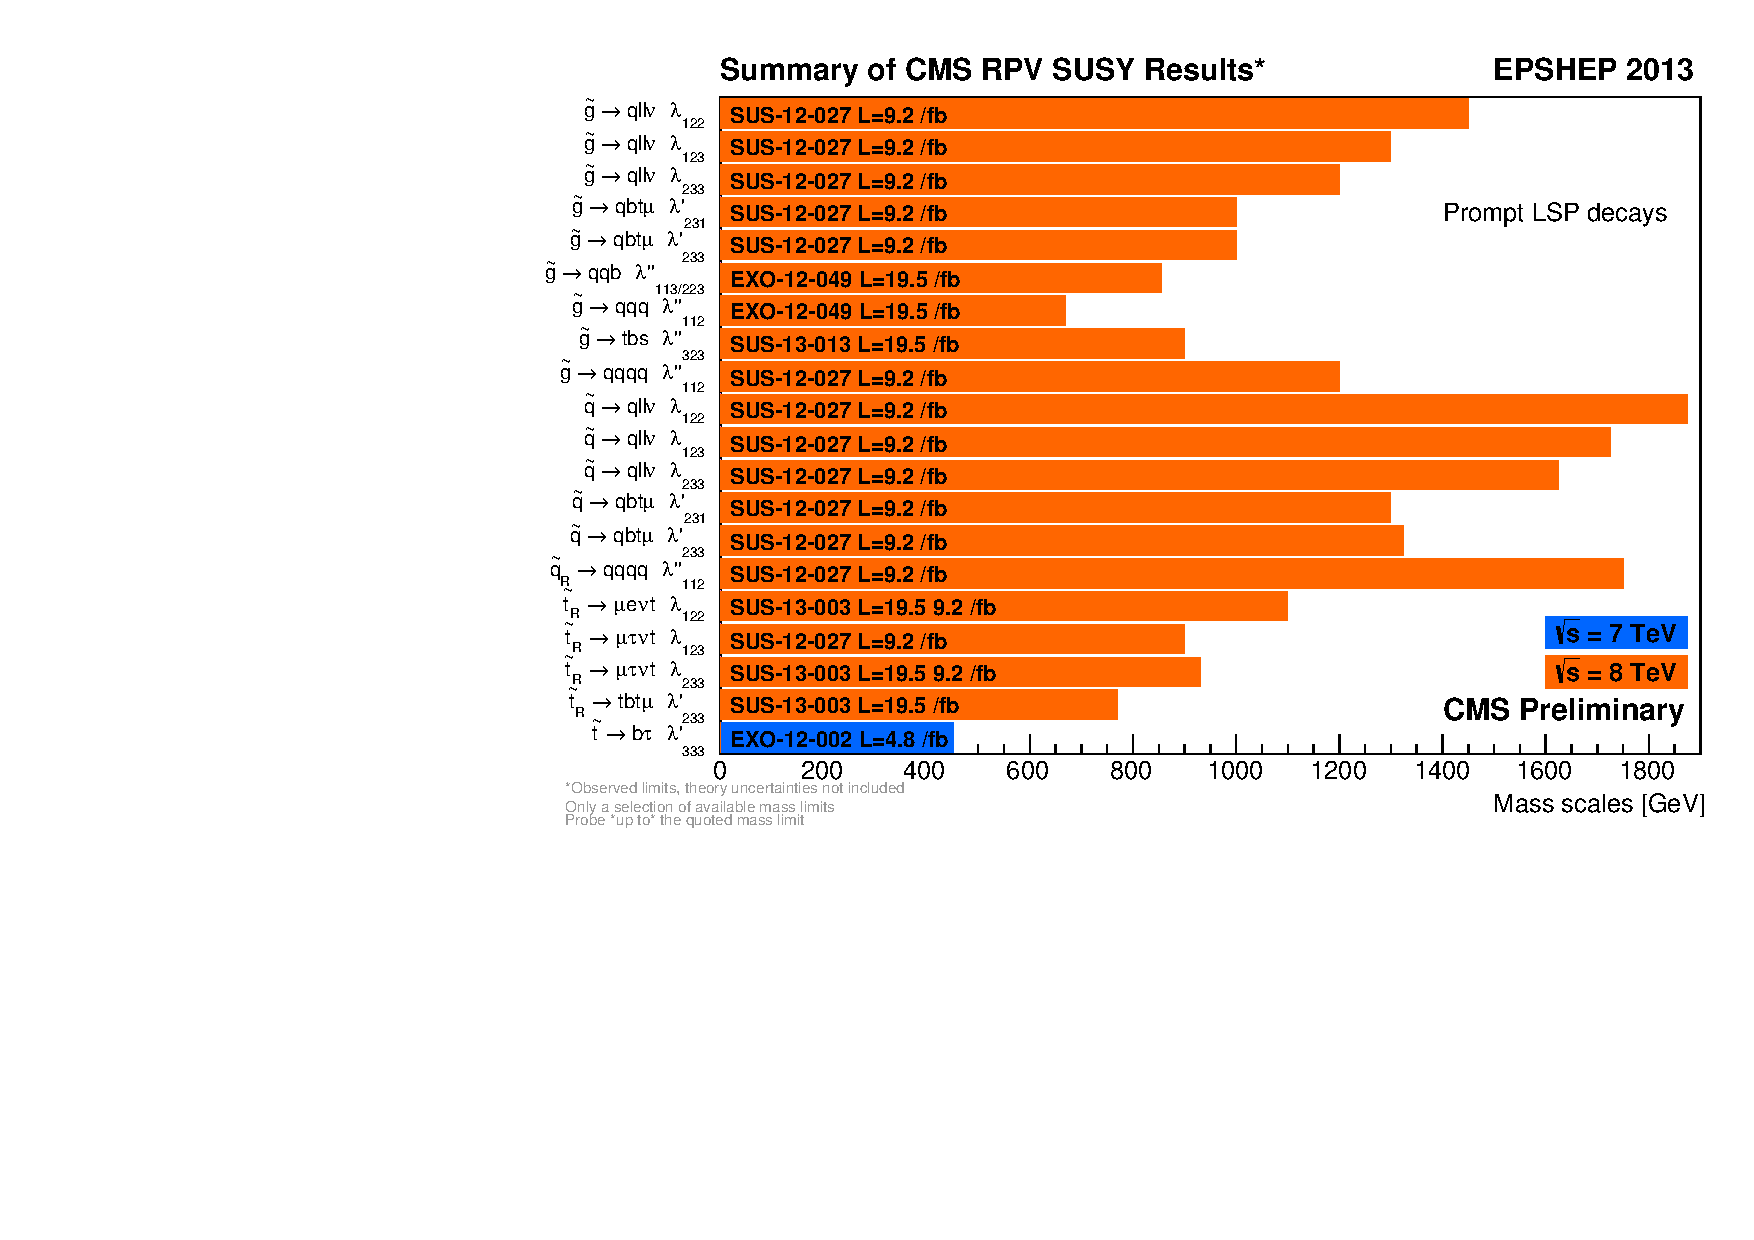
\includegraphics[width=0.9\textwidth]{Images/Introduction/RPVbarplot_blue_orange_EPSHEP2013.pdf}
	\caption{Best exclusion limits for the masses of the mother particles, for RPV scenarios, for each topology, for all results. In this plot, the lowest mass range is $m(\text{mother})=0~\si{GeV}$, but results are available starting from a certain mass depending on the analyses and topologies. Branching ratios of one are assumed, values shown in plot are to be interpreted as upper bounds on the mass limits \cite{cms_results}.}
	\label{fig:MODEL_DEPENDENT_2}
\end{figure}

However, the current techniques used in hep fail to capture all of the available information, as proved by \cite{baldi}. The recent developments in Deep Learning theory can overcome these issues. (Deep) Neural networks provide powerful classifiers and can also solve the curse of high dimensionality of data. Moreover, circuit complexity theory has proved that deep neural networks have the potential to compute in an unbiased way arbitrary complex functions in a very efficient way. Employing them to parametrize alternative distributions for model-independent new physics searches is thus a highly motivated attempt.

Several approaches with neural networks to the problem of new physics research have been developed so far, starting from the one given by \cite{baldi}. The approach employed in this thesis work is introduced by \cite{wulzer}. Technically speaking, we can exploit neural networks to find an anomalous behavior, relative to the reference model, of the entire data sample, with which we train the network. The process studied is the decay of the $Z$ boson into a pair of muon-antimuon, assuming for new physics events different kind of signals in order to test the efficiency of the approach.

\vspace{5mm}
\noindent
The content of this thesis work is ordered as follows:
\begin{itemize}
	\item In Chapter \ref{chap:NN} a general recap on deep learning theory and on neural networks is given. Common practices in the training procedure are explained too.
	\item In Chapter \ref{chap:LHC} LHC collider is described along with CMS experiment. In particular, in Chapter \ref{chap:Z} a summary on the process analyzed can be found.
	\item In Chapter \ref{chap:Z_5D} the algorithm employed for anomaly detection is explained and in Chapter \ref{chap:W_CLIP} a necessary tuning procedure is illustrated. Finally, the results are presented in Chapter \ref{chap:RESULTS}.
	\item In the final Chapter \ref{chap:CONCLUSION} possible developments of the method and of the algorithm are provided.
\end{itemize}